% !TeX encoding = UTF-8
% !TeX root = ../Vitamintablettenspender.tex

\chapter{Methodische Werkstoffauswahl}
Von der Produktentwicklung werden leistungsfähige Systeme bei gleichzeitiger Erfüllung von Sicherheits- und Umweltverträglichkeitsanforderungen erwartet. Steigenden Kosten für Material und Energie werden im Zuge des Multi-Material-Designs mittels einer methodischen Werkstoffauswahl durch die \glqq Ashby-Methode\glqq{} und den dabei entstehenden intelligenten Lösungen entgegengewirkt. Dabei werden unterschiedlichste Aspekte wie die Möglichkeit zur generativen Fertigung bzw. dem Additive Manufacturing berücksichtigt. Die Auslegung der Hauptkomponenten des Produktes unterliegt den jeweils gültigen Randbedingungen und ihren zu erfüllenden Funktionen und werden hinsichtlich ihrer freien Variablen untersucht und bezüglich der Werkstoffauswahl optimiert. Eine \glqq Performance-Rechnung\grqq{} ermöglicht die Einbeziehung von mathematischen und physikalischen Formeln zur Entmystifizierung der Werkstofffaktoren. In der kommerziellen Software CES Selector der Firma Granta Design Ltd. (Cambridge, Vereinigtes Königreich), die von Michael Ashby, dem Erfinder der Ashby-Methode, gegründet wurde, wird mittels einer computergestützten Datenbank auf Basis der Performance-Rechnung die fünf besten in Frage kommenden Werkstofflösungen ermittelt, woraus die optimale Werkstofflösung durch \glqq weiche\grqq{} Faktoren resultiert.\\
Für die Anwendung der Ashby-Methode muss zunächst die Hauptfunktion des Bauteils bestimmt werden. Darauffolgend müssen Randbedingungen sog. Constraints definiert werden, auf Basis derer ein Ziel zur Optimierung gesetzt wird. Dabei treten freie Variablen auf, die während des Designprozesses des Produktes variiert werden können. Die Randbedingungen liefern im Allgemeinen numerische Gleichungen die einen Performance-Index implizieren. Ein höherer Performance-Index bedeutet konventionell ein besseres Material.\\
Im Folgenden wird das Prinzip von Ashby zur Materialauswahl auf die vier Hauptkomponenten des Systems angewandt.

\section{Standfuß und Gehäuse}
Das Gehäuse inklusive des Standfußes ist im Querschnitt zusammen mit den wesentlich angreifenden Lasten in Abb. \ref{fig:0301skizze} (a) dargestellt. Die Streckenlast $q_0$ fasst die Gewichtskräfte des Tablettenauswurfs, der Aktoren sowie der Behälter für die Lagerung der Tabletten zusammen. Die Einspannung am unteren Ende symbolisiert die Lagerung des Bauteils an der Oberfläche. Eine geeignete Abstraktion des Systems wird durch die Reduzierung der Streckenlast sowie der Einspannung auf zwei resultierende Kräfte in \ref{fig:0301skizze} (a) beschrieben. Darin ist die Kraft $F_{res}$ die Resultierende aus der Streckenlast und greift im Schwerpunkt der Last an. Die Einspannung am unteren Ende reduziert sich zu der für die Berechnung wesentlichen vertikalen Komponente $F_{L,V}$. Unter Vernachlässigung des Eigengewichts des Bauteils gilt näherungsweise $F_{res}\,\approx\,F_{L,V}$. Die Werkstoffauswahl und die Optimierung einer Zielfunktion kann für den dargestellten kritischen Teil des Gehäuse stellvertretend für die gesamte Struktur vorgenommen werden.
\begin{figure}[H]
	\centering
	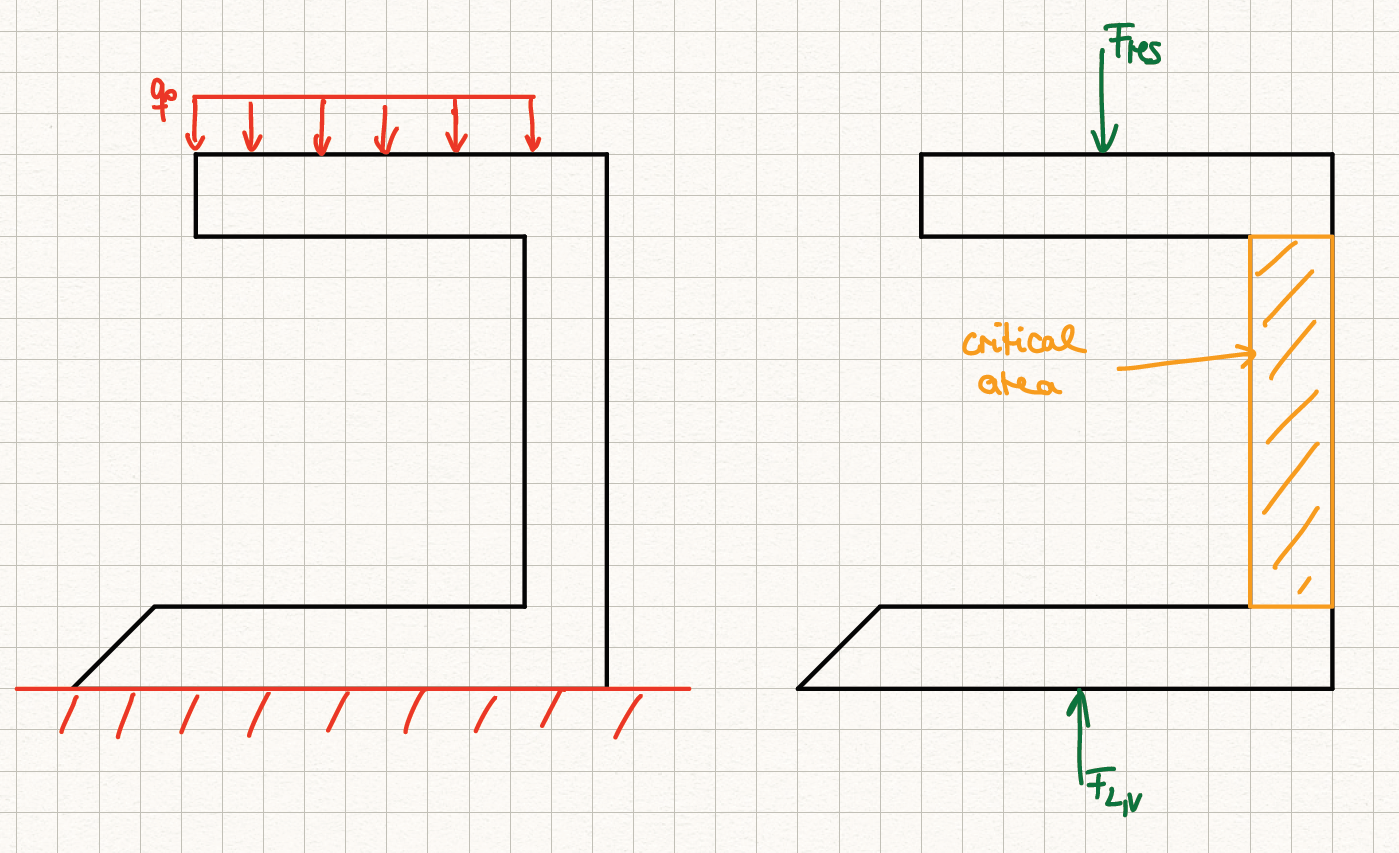
\includegraphics[width=1.0\linewidth]{chapter/Bilder/0301skizze}
	\caption{(a, links) Querschnittsdarstellung des Gehäuses und angreifende Lasten, (b, rechts) vereinfachte Darstellung mit angreifenden resultierenden Kräften und der kritischen Zone}
	\label{fig:0301skizze}
\end{figure}
\begin{figure}[H]
	\centering
	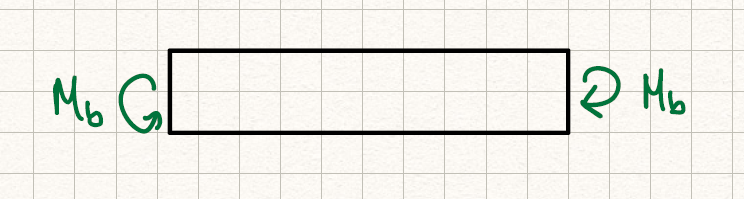
\includegraphics[width=1.0\linewidth]{chapter/Bilder/0301modell}
	\caption{Abstrahiertes Modell einer Platte unter reiner Biegung mit dem Biegemoment $M_b$}
	\label{fig:0301model}
\end{figure}
Dabei ist die \textbf{Funktion} des Bauteils den Tablettenauswurf, die Aktoren sowie die Tablettenbehälter zu stützen und in der Höhe zu halten. Auf Basis der Anforderungsliste in \ref{anforderungsliste} und der benötigten mechanischen Eigenschaften können folgende \textbf{Randbedingungen/Constraints} definiert werden:
\begin{itemize}
	\item Material muss recyclebar sein
	\item Höhe des kritischen Teils/Länge der Platte $L\,=\,180\,$mm
	\item Material muss ein guter Isolator sein, bzw. $\rho_e\,>\,10^{19}\,\mu\Omega$cm
	\item CO$_2$-Ausstoß bei der Materialgewinnung $<\,2\,\frac{kg\,(\text{CO}_2)}{kg\,(\text{Material})}$
	\item Biegesteifigkeit $S$ so, dass bei Einleitung der Kraft $F_{res}$ das an der Platte resultierende Biegemoment $M_b$ eine maximale Durchbiegung $w_{\text{max}}$ zur Folge hat
\end{itemize}
Das \textbf{Ziel} der Werkstoffauswahl ist die Reduzierung der Kosten für das Gehäuse. Als \textbf{freie Variablen} treten dabei zum einen die Querschnittfläche der rückwandigen Platte, welche durch Konzeptleichtbau im Verlauf des Produktdesigns optimiert werden kann, zum anderen die Wahl des Materials.
Dadurch, dass die Biegesteifigkeit $S$ sowie die Höhe der Platte $L$ vorgegeben sind, ergeben sich die beiden Gleichungen als Grundlage der Performance-Rechnung. Hierbei gilt zunächst für die Durchbiegung in der vertikalen Mitte der Platte ausgehend von der Differentialgleichung 2. Ordnung:
\begin{equation}
	E\,I\,w''(x)\,=\,-\,M_b\,
\end{equation}
durch zweifaches Integrieren, Umstellen und Einsetzen unter Vernachlässigung des Vorzeichens, das ausschließlich für die Richtung der Durchbiegung berücksichtigt werden muss:
\begin{equation} \label{durchbiegung}
	w\,\left(\frac{L}{2}\right)\,=\,\frac{M_b \,L^2}{8\,E\,I}\,\le\,w_{\text{max}},
\end{equation}
wobei $E\,I$ der Biegesteifigkeit $S$ entspricht. Als weitere Gleichung ergibt sich der Zusammenhang für die effektiven Kosten $K$, die in erster Linie über den Kostenfaktor $C_m$ mit der Masse der Platte korrelieren. Unter Berücksichtigung der Geometrie und der Materialdichte $\rho$ ergibt sich:
\begin{equation} \label{kosten}
	K\,=\,C_m\,m\,=\,C_m\,\rho\,A\,L\,.
\end{equation}
Dabei ist das Flächenträgheitsmoment eine Funktion der Querschnittfläche, die als rechteckig angenähert werden kann. Hier sind jedoch die Kantenlängen $h$ und $b$ variabel. Damit gilt für die Querschnittsfläche:
\begin{equation} \label{flächeninhalt}
A\,=\,h\,b
\end{equation}
sowie für das Flächenträgheitsmoment:
\begin{equation} \label{flächenträgheitsmoment}
I\,=\,\frac{h\,b^3}{12}\,.
\end{equation}
Einsetzen von \ref{flächenträgheitsmoment} in \ref{durchbiegung} und \ref{flächeninhalt} in \ref{kosten} liefert die Gleichungen:
\begin{equation} \label{eingesetzt}
	w_{\text{max}}\,\ge\,\frac{3\,M_b \,L^2}{2\,E\,h\,b^3}\,, \qquad
	K\,=\,C_m\,\rho\,h\,b\,L
\end{equation}
Eliminieren von $b$ führt in \ref{eingesetzt} schließlich zu
\begin{equation}\label{performance}
K\,=\,\underbrace{\left(\frac{3\,M_b\,L^5\,h^3}{2\,w_{\text{max}}}\right)^{\frac{1}{3}}}_\text{vorgegeben, bzw. geometrieabhängig}\,\frac{C_m\,\rho}{E^{\frac{1}{3}}}\,.
\end{equation}
Damit ist die \textbf{Zielfunktion} mit
\begin{equation} \label{zielfkt1}
P_{\text{CR}}^{3.1}\,=\,\frac{1}{K}\,=\,\frac{E^\frac{1}{3}}{C_m\,\rho}
\end{equation}
definiert, wobei $P_{\text{CR}}^{3.1}$ zu maximieren ist.\\
CES-materialselection ...

\section{Tablettenrutsche}
Die Tablettenrutsche besitzt die wesentliche \textbf{Funktion} die aus der Lagerung geschobenen Vitamintabletten mittels Schwerkraft entlang einer Bahn in ein bereitgestellten Trinkbehälter zu überführen. Für die Werkstoffauswahl liegen folgenden \textbf{Randbedingungen/Constraints} vor:
\begin{itemize}
	\item Material muss generativ bzw. additiv fertigbar sein
	\item Material muss recyclebar sein
	\item Plattengeometrie: Trapezförmiger Querschnitt (gleichschenklig und symmetrisch, Grundseite $l_1\,=\,34\,$mm, Grundseite $l_2\,=\,100\,$mm, Höhe $h\,=\,40\,$mm)
	\item Plattendicke $3\,=\,mm$
\end{itemize}
Das \textbf{Ziel} der Werkstoffwahl liegt in der Minimierung des CO$_2$-Ausstoßes bei der Materialgewinnung unter Erfüllung der minimalen spezifischen Festigkeit, die gewährleistet, dass trotz der hohen Zahl an Auswurfzyklen die Bauteilstruktur nicht beeinflusst wird. \textbf{Freie Variable} ist in dem Auslegungsprozess die Wahl des Materials.\\
Aufgrund der vorgegebenen Plattengeometrie gilt für den CO$_2$-Ausstoß beim Materialgewinnung
\begin{equation}
\text{CO}_2^{ges}\,=\,\text{CO}_2\,m\,=\,\text{CO}_2\,\rho\,V\,=\,\text{CO}_2\,\rho\,A\,d\,=\,\text{CO}_2\,\rho\,\frac{1}{2}\,(l_1\,+\,l_2)\,h\,d\,.
\end{equation}
Für die Bruchlast gilt bei Biegebeanspruchung der Platte:
\begin{equation}
F_B\,=\,C\,\frac{I\,\sigma_f}{y_m\,h}\,
\end{equation}
dabei ist $C$ eine Konstante, die abhängig von der genauen Belastung ist. Da der Belastungszustand jedoch sehr variabel ist und für die nachfolgende Rechnung nicht näher spezifiziert 
Masse mit Energie in der Produktion als Faktor zu Dichte\\
\begin{equation} \label{zielfkt2}
P_{\text{CR}}^{3.2}\,=\,\frac{\sigma_f^\frac{1}{2}}{\text{CO}_2\,\rho} (Seite 510 ca)
\end{equation}

\section{Tablettenlagerung}

Die \textbf{Funktion} dieses Bauteils stellt das sichere Lagern der Vitamintabletten sowie dem Zulassen einer optischen Prüfung des Füllstandes dar. Zur Erfüllung dieser Funktion sind folgenden \textbf{Randbedingungen/Constraints} gegeben:
\begin{itemize}
	\item Material muss durchsichtig/transparent sein
	\item Bauteilhöhe $l\,=\,200\,$mm
	\item Innenradius des Lagerungszylinders $r\,=\,14\,$mm
	\item Steifigkeit: Kein Umknicken bei Befüllung
	\item Festigkeit: Keine plastische Verformung bei Befüllung
	\item CO$_2$-Ausstoß bei der Materialgewinnung $<\,2\,\frac{kg\,(\text{CO}_2)}{kg\,(\text{Material})}$
\end{itemize}
Das \textbf{Ziel} der Werkstoffauswahl ist die Minimierung des Produktionsenergie für eine ausreichende Biegesteifigkeit. \textbf{Freie Variable} ist die Wahl des Materials.\\
Biegebalken aber mit Querschnitt für Rohr\\
Masse mit Faktor für C02 zu Dichte
\begin{equation} \label{zielfkt3}
P_{\text{CR}}^{3.3}\,=\,\frac{E^\frac{1}{2}}{E_p\,\rho} (Seite 432 Beam)
\end{equation}